\section{Analyse der Logdaten}
\label{chap:log_analysis}

Wie in Abschnitt~\ref{chap:evaluation} beschrieben,
werden Nutzerinteraktionen durch das Loggingsystem erfasst.
Das so gesammelte Feedback kann auf zweierlei Weise analysiert werden.
Mittels Online-Analyse kann der Index um neue Daten erweitert oder Einfluss auf das Ranking ausgeübt werden.
So kann die Menge der Query Suggestions mit Hilfe der durch Nutzer gestellten Anfragen erweitert werden.
Außerdem kann die Häufigkeit von Suchbegriffen auch mit Bezug zum zeitlichen Kontext das Ranking beeinflussen,
um populäre Vorschläge weiter vorn zu listen.
Da die Links der SERP zudem Tracking erlauben, kann ermittelt werden,
welche Ergebnisse tatsächlich von den Nutzern angeklickt werden, und welche Ergebnisse eher irrelevant sind.
Für das Tuning der Suchmaschine ist im Gegensatz dazu eine Offline-Auswertung vorzuziehen.
Zu diesem Zweck können die Sessions ausgewählter Testnutzer ausgiebig protokolliert werden,
um Metriken wie Precision und Recall zu ermitteln.
Die in diesem Kontext durchgeführte Evaluation wird im folgenden Abschnitt beschrieben.

\subsection{Durchführung eines Laborexperiments}
\label{chap:labroratory_experiment}

Um Schwächen der Suchmaschine zu identifizieren sowie die Effektivität von Parametertuning bewerten zu können, muss die Ergebnisqualität mit Hilfe verschiedener Metriken erfasst werden. Dabei ist es vergleichsweise einfach, die Precision zu bestimmen, indem die Relevanz einzelner Treffer in den Ergebnismengen beurteilt wird. Da allerdings die Menge der tatsächlich relevanten Dokumente zu einer Suchanfrage nicht bekannt sind, kann der Recall-Wert nur approximativ ermittelt werden.

Aus diesem Grund wird ein initiales Experiment durchgeführt, bei dem Testnutzer die ersten 30 Suchergebnisse zu vorgegebenen Topics nach deren Relevanz bewerten. Zu Beginn werden 50 entsprechende Suchanfragen sowie deren Information Need und die Relevanzkriterien vorbereitet. Im Anschluss werden die Suchen durchgeführt und für jedes Ergebnis auf den Rängen 1 bis 30 erfasst, ob ein Ergebnis irrelevant oder relevant ist bzw. ob dieses exakt das gewünschte Dokument darstellt. Auf diese Weise wird zu jedem Topic ein Korpus relevanter Dokumente erstellt, welcher zudem manuell um noch nicht enthaltene Ergebnisse erweitert werden kann. In nachfolgenden Experimenten kann diese Suche sowie die Bewertung dann automatisiert auf Basis der so erhobenen Daten durchgeführt werden. Damit ist eine schnelle Bewertung von Parameteränderungen möglich.

\begin{figure}[!ht]
	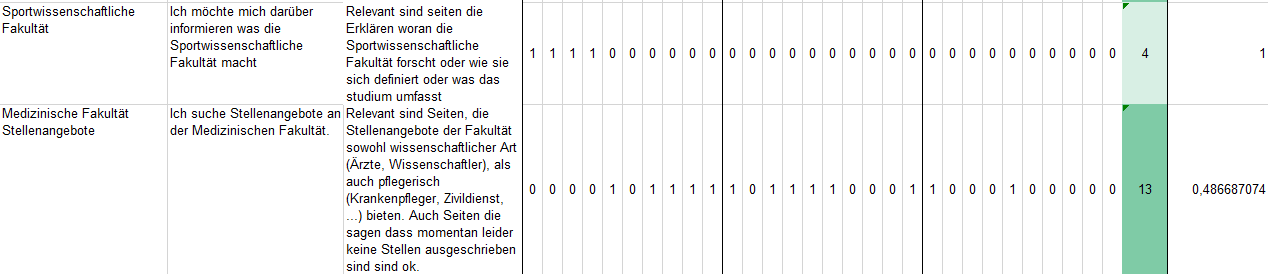
\includegraphics[width=0.99\textwidth]{chapter_log_analysis/evaluation_topics.png}
	\caption{Überblick über einen Teil der Topics des Laborexperiments}
	\label{fig:labroratory_experiment}
\end{figure}



Im Rahmen der Durchführung der Bewertungen haben sich einige Auffälligkeiten gezeigt, die im Folgenden kurz erläutert werden: 

\begin{description}

\item In den Ergebnissen tauchen häufig Seiten bestimmter Fakultäten beziehungsweise Institute auf, weil Wortwahl und Struktur der Webpräsenz das Ranking der Seite besonders positiv beeinflussen. Im Gegensatz dazu stehen andere Websites, welche über verschiedene URLs erreichbar sind oder für jedes Semester dieselben Informationen in abgewandelter Form veröffentlichen und damit die Bewertung ihrer einzelnen Seiten herabsetzen.

\item Weiterhin ist anhand der Ergebnisse ersichtlich, dass die Suchmaschine der Reihenfolge der Suchbegriffe innerhalb der Query stark überbewertet. So werden Dokumente, welche das erste Wort mehrfach enthalten noch vor jenen gelistet, welche alle Suchbegriffe enthalten.

\item Darüber hinaus wird klar, dass häufig aufgrund anderer Schreibweisen, Abkürzungen oder einfach nur Synonymen das gewünschte Ergebnis nicht gefunden werden kann. Da es sich häufig um fachspezifische Terminologien handelt, ist die Standardkonfiguration der Suchmaschine nicht ausreichend.

\item Ein Fall, bei dem der gesamte Inhalt eines PDF-Dokuments als Bild eingebettet ist, zeigt außerdem die Limitierungen der zur Indexierung verwendeten Software. Da diese kein OCR anwendet, ist der gesamte enthaltene Text nicht im Index zu finden.

\end{description}

Die Auswertung der Metriken zeigt, dass in den MRR-Szenarien bei rund 63\% der Anfragen das gesuchte Ergebnis innerhalb der Top 10 zu finden ist. Bei einer weiteren Anfrage wird Rang 14 erreicht. Bei allen weiteren Anfragen (etwa ein Drittel) kann das gesuchte Dokument nicht innerhalb der ersten 30 Suchergebnisse gefunden werden.
 
In den 24 nicht-MRR-Szenarien, bei denen nicht nur ein bestimmtes Dokument gesucht wird, zeigen sich ähnlich unterschiedliche Ergebnisse. Neben einzelnen Anfragen, die die meisten Spitzenplatzierungen mit relevanten Dokumenten besetzen, existieren auch drei Szenarien, die in ihrer Ergebnismenge kein einziges als wichtig erachtetes Dokument enthalten. Die meisten Resultate liegen dagegen jedoch im Mittelfeld, sodass sich insgesamt eine Mean Average Precision von \textasciitilde 0,535 ergibt.
